\documentclass{article}
\usepackage{graphicx} % Required for inserting images
\usepackage{hyperref}
\usepackage[backend=biber,style=numeric,]{biblatex}
\title{MINECRICKET}
\author{Anoop Amarapu \\ roll. no. 22B1011}
\date{June 2023}
\addbibresource{report.bib}
\begin{document}

\maketitle

\section{Introduction}
This is a basic game which is written in HTML, CSS and JavaScript. I named it the 'MINECRICKET' inspired from the classic minesweeper game and cricket.

\section{Code explanation}
The code  basically is a combined effect of three different code snippets, one of HTML, one of CSS and the third of JavaScript.\\

HTML code, named as minecricket.html, contains the elementary tags including the headings, titles, etc. and the tags which import CSS and JavaScript code snippets to render its effect.\\

CSS code, named as minecricket.css, contains all the designing and styling effects to the final web-page. It employs facilities like background image inclusion, grid construction, placing of the web-page text in the final web-page, etc..\\

JavaScript code, named as minecricket.js, serves the intelligence of the game, the intellectual functionality of the game, etc..\\

\begin{figure}[!ht]
    \centering
    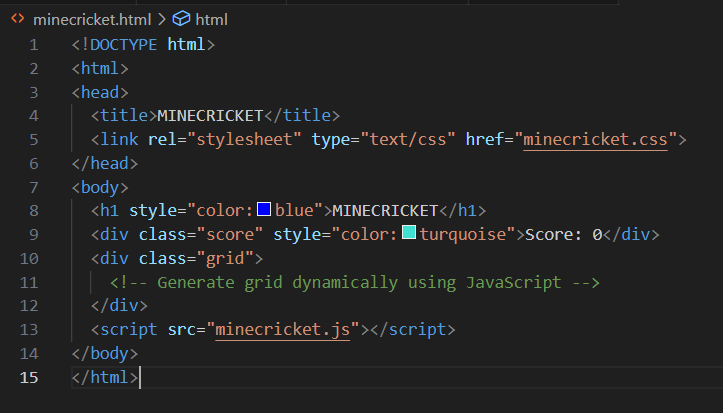
\includegraphics[width=0.5\textwidth]{html.png}
    \caption{The HTML code snippet}
    \label{fig:image}
\end{figure}

\begin{figure}[!ht]
    \centering
    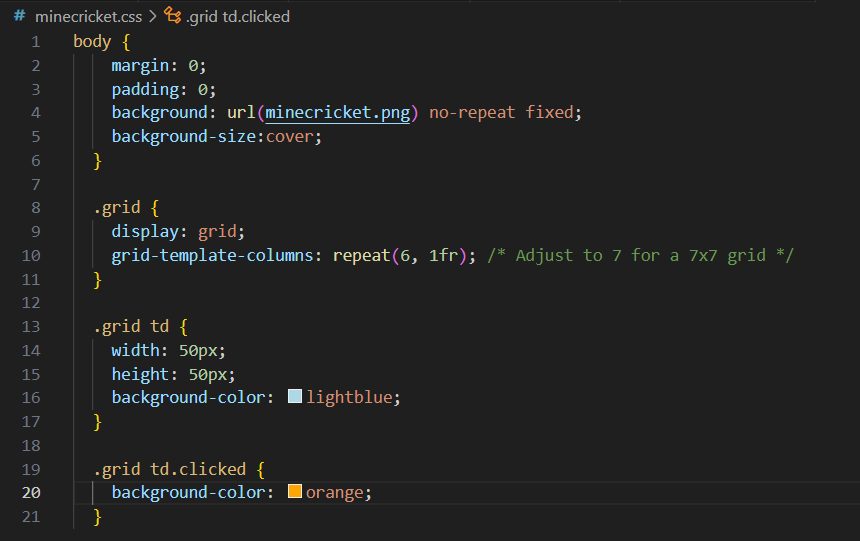
\includegraphics[width=0.5\textwidth]{css.png}
    \caption{The HTML code snippet}
    \label{fig:image}
\end{figure}

This CSS code snippet consists of all the styling properties of the final web-page to be rendered. The background image is included in the style part of body. A classes are used in here, '.grid' used to point to the grid construction. '.grid td' is used for specifying the dimension of each grid cell and finally '.grid td.clicked', helpful in changing the features of the cell grid after it is clicked.\\
    
\begin{figure}[!ht]
    \centering
    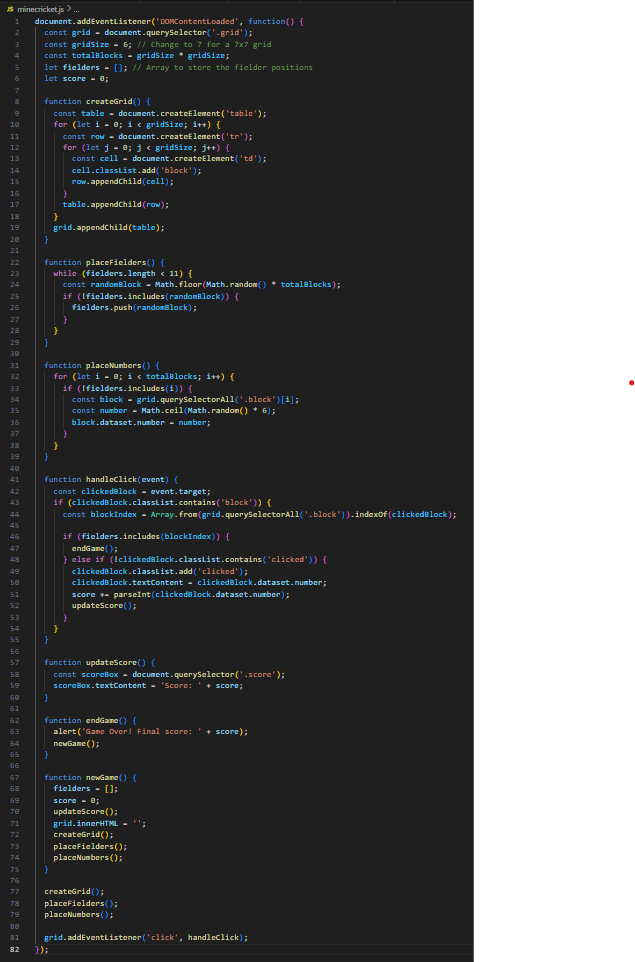
\includegraphics[width=0.5\textwidth]{js.png}
    \caption{The HTML code snippet}
    \label{fig:image}
\end{figure}

The JavaScript code plays the role of intelligent code in here.\\

1] DOMContentLoaded event:

The code is wrapped in an event listener for the DOMContentLoaded event, which fires when the initial HTML document has been completely loaded and parsed.\\

2] Variables:

a) grid: It represents the DOM element with the class grid which will contain the game grid.
b) gridSize: It represents the size of the grid. By default, it is set to 6, but you can change it to 7 to have a 7x7 grid.
c) totalBlocks: It represents the total number of blocks in the grid, calculated by multiplying gridSize by itself.
d) fielders: It is an array that stores the positions of the fielders (blocks that should be avoided by the player).
e) score: It holds the current score of the player.\\

3] createGrid() function:

This function dynamically creates a table-based grid with gridSize rows and columns. It creates gridSize number of <tr> elements and gridSize number of <td> elements within each row to form the grid structure. Each <td> element is given the class block for styling.\\

4] placeFielders() function:

This function randomly selects positions (fielders) in the grid where the fielders (blocks to be avoided) will be placed.
It ensures that there are exactly 11 fielders in total.\\

5] placeNumbers() function:

This function assigns a random number between 1 and 6 to each block that is not a fielder. It uses the dataset property of each block element to store the assigned number.\\

6] handleClick() function:

This function handles the click event on the grid. It checks if the clicked element has the class block to ensure that it's a valid block in the grid. It determines the index of the clicked block using Array.from() and indexOf(). If the clicked block is a fielder, the endGame() function is called. If the clicked block is not already clicked, it adds the clicked class, displays the assigned number, updates the score, and calls the updateScore() function.\\

7] updateScore() function:

This function updates the score displayed on the webpage by selecting the element with the class score and modifying its textContent property.\\

8] endGame() function:

This function is called when a fielder is clicked, indicating that the game is over. It displays an alert with the final score and then calls the newGame() function to start a new game.\\

9] newGame() function:

This function resets the game state to start a new game. It clears the fielders, resets the score, updates the score displayed, clears the grid, and recreates the grid, places fielders, and assigns random numbers to non-fielder blocks.\\


10] Event listeners:

The DOMContentLoaded event listener wraps the entire code to ensure that the code execution starts after the HTML document has been loaded. The click event listener is added to the grid element to handle clicks on the grid. It calls the handleClick() function.\\

\section{References}
I have used 3 cites as references for my project. \cite1 for getting the broad understanding of the basic simulation of the code, which is necessary so that I can make customized alterations to any source code I procure and to fix bugs, if any. \cite2 for learning the styling part of the code. \cite3 as the source of images in the background.
\printbibliography



\end{document}



